\documentclass{article}
\usepackage[utf8]{inputenc}
\usepackage{multicol}
\usepackage[margin={1.25in,1.25in}]{geometry}
\usepackage{titlesec}
\usepackage{titling}
\usepackage{graphicx}
\usepackage{stfloats}
\usepackage[
    backend=biber,
    style=ieee,
    url=false, 
    doi=false,
    eprint=false
]{biblatex}

\usepackage{parskip}

\title{Final Paper}
\author{Ryan Bruno}
\date{\today}

\addbibresource{bib.bib}

\renewcommand{\maketitle}{
    \begin{center}
        \Huge\textbf{\thetitle}
    \end{center}
    \begin{multicols}{2}
        \begin{flushright}
        By: \theauthor
        \end{flushright}

        \columnbreak
        
        \thedate
    \end{multicols}
}

\begin{document}

\maketitle

\begin{multicols}{2}
\begin{refsection}
%\large

\section*{Abstract}

While the cost of digital storage is at an all-time low, data
accumulation of unnecessary replication metadata comes at a cost.
Conflict-free Replicated Data Types are being used to ensure
eventual consistency throughout a distributed system but many proposed
solutions do not take into account memory consumption and simply allow for
an unbounded metadata growth. In this paper, we explore two methods of
memory reduction in the form of garbage collection.

\section*{Introduction}

In order to maintain data availability, large-scale systems not only
have to keep multiple copies of their data on different nodes but they
must also allow nodes to make changes or make decisions based on that
data without a quorum of nodes being available. This leads to variance
among nodes and in the past developers would have to create their own
algorithms to handle data invariance manually \cite{kleppmann_conflict-free_2017}.
It was clear that a solution needed to be described in a way that
developers who are already familiar with textbook abstract data types
could understand and use. This leads us to an abstraction that builds
upon textbook abstract data types but provides certain guarantees to avoid
distributed conflicts called Conflict-Free Replicated Data Types (CRDTs).
CRDTs provide the guarantee that when two or more nodes merge they will
always end in the same state at that point in time. It is also guaranteed
that synchronous writes will both be kept in a merge; meaning no write
ever gets lost \cite{shapiro_comprehensive_2011}.

\section*{Literature Review}

\subsection*{System Description}

To start we will first describe the types of systems that are applicable
for the use of CRDTs. The primary two targets are large-scale systems
and limited connectivity devices. Large-scale systems are those deployed
by large web-services or companies that must serve many clients spread
all around the globe \cite{tao_merging_2015} \cite{balegas_making_2016}.
The amount of nodes in those systems grows and shrinks rapidly therefore
we assume the amount of total amount of nodes in the system at any point
in time is not known, nor can we rely on any type of quorum to be
present to make decisions. The second type of system includes limited
connectivity devices. This could be a mobile device for which it's user
can make changes to data locally but, with an unreliable network
connection, the application is not expected to be able to sync with a
server in order to make those changes \cite{perkins_simba:_2015}. Some
other system requirements are listed below:

Node: We assume all nodes can connect at some point in the future and
are synchronous; so they can communicate, merge, and change data in
distinctly different periods of time.

Data: A piece of data, unless otherwise specified, is assumed to be
immutable and has no relationship to other data. We leave up to
implementation how to generate a view of the data as it should not
affect the merging algorithm.

Merge: The CRDTs described here are state-based CRDTs as opposed to
operation-based CRDTs. During the merge of a state-based CRDT, we
assume one node sends its entire data set to another where it is merged
with the target's data set \cite{shapiro_comprehensive_2011}.


\subsection*{Grow-Only Set}

One of the most simple CRDTs is a set that only has an add operation. In
math, a set has two operations add() and remove(). If we allow both
these two operations a problem arises when merging two nodes as we
cannot determine which node has the most up-to-date data. For example,
if node A deletes an element then, to stay consistent in a merge, node B
should delete that element as well. However, what should happen if
before the merge node B removed the element then added it back? Without
any metadata node A and node B have no way of knowing what operation is
most up to date; the removed item or the added back item. With that in
mind, the easiest solution is to not allow the remove operation at all
\cite{shapiro_comprehensive_2011}. It may sound useless but grow-only
sets are deployed in a lot of places from logs to your bank account;
which is nothing more than a set of transactions that cannot be removed
(in the event of a chargeback a new reversal transaction is added).
Being one of the most simple CRDTs it is also the most simple to prove.
The merging semantics of a Grow-Only set is a simple union which is a
commutative operation; meaning both nodes will end in the same state.
Lastly, due to the way we chose to represent data synchronous adds are
not a problem.

\subsection*{Two-Phase Set}

Building off the previous problem, 
Given the problem introduced previously we understand that conflicts
arise when a node deletes an item but an algorithm cannot determine if
the item should be deleted or, in the case of another node adding the
item back after it was deleted, it should stay. This leads us to the
next solution which is to allow adds and removes but once an item is
removed it cannot be added back \cite{shapiro_comprehensive_2011}. This
is called a Two-Phase Set or 2P-Set and is accomplished using tombstones.
When a node deletes an item it sets a special marker on that item
telling all other nodes to delete that item forever. The merge algorithm
is similar to a set union except each item should carry a tombstone flag
with it. The new tombstone flag for a given item should be a bitwise OR
operation of the tombstone flag for that item in each set.

\subsection*{OR-Set}

The idea of an OR-Set builds on the previous logic asking ``can we get
around the re-add restriction by adding a unique id to each added item?"
An OR-set automatically adds a unique id to every item that is added to
the set and this alone lifts any restrictions on the add or remove
operations \cite{shapiro_comprehensive_2011}. We no longer run into the
problem of removing and adding the same item due to the fact that every
added item is different because of the unique id. Now we have a CRDT
that has no restrictions on the add or remove function; similar to a
math set. We can guarantee that all sets will merge without any conflicts
as long as the ids are unique. An application can now also update data in
the set by simply removing an item, changing it, then adding it back.
Traditional developers may ask the question ``What happens when two nodes
change a value at the same time?" The answer is that both values will be
left in the set. CRDTs are conflict-free in their merge operation but
may be left in a state of conflict from the application's standpoint.
This leaves the developer to handle these types of conflicts.

\subsection*{Relationships}

In order to allow for the easy transition from relational database
schema, we can provide a mechanism for handling relationships in a
distributed environment. We can provide such this mechanism with two
changes \cite{balegas_making_2016}. To exemplify these changes lets
begin with a one-to-many relationship between managers and employees.
If a node would like to add a new employee under a manager the node
would add to the set both the employee, the manager, and the
relationship between them. This is the first change and provides the
foreign key integrity constraints that are familiar in most relational
databases as a synchronous delete of the manager would be canceled out
by the addition of the manager back into the set. This type of merge is
called ``last writer wins" and may not be ideal for some situations for
example if we really want to delete a manager. In order to do this, we
create a new set used by the merging algorithm. In our example, if we
would like to delete manager ``m" we tell the merge algorithm to drop
every item matching ``m" and relationship R(m,*). This would not allow
the manager nor any relationship with the manager to return. To recap:
The data and relationships can be represented by either a Grow-Only, 2P
or Or-Set. Their add operation, if applicable, would work the same while
their remove operation would include additional logic to ensure
relationships are removed. The merge algorithm may use an additional set
to track deleted relationships and items (in the case of a cascading
delete).

\subsection*{Garbage-Collection}

OR-Sets are great in many ways but one of its drawbacks is the unbounded
accumulation of tombstones. The only job of a tombstone is to ensure the
deletion of an item in other nodes and once every node has seen the
tombstone it can be safely be deleted from every node \cite{bauwens_memory_2019}.
There are two solutions to this problem that can both be used
simultaneously. Both solutions require us to force our system to have a
known finite number of nodes and must ensure local operation ordering.
The first solution piggyback on the idea that tombstones may be deleted
when they are no longer needed and operation ordering. A single node will
ignore tombstones originating from another if the latest item it has
received from the originating node is grater then the item in question.
This prevents incorrect reappearance of items and allows nodes to remove
a tombstone once it has received it from the nodes where it has originated.
A node can choose to delete a tombstone as soon as it receives it
from its origination node or first relay it to other peers for a set
period of time. The second solution trades collection rate for network
overhead. If an originating node broadcasts an operation it must hear
back from each node for the operation to be ``casually stable". This
may take a while as nodes could be buffering responses. Eager collection
speeds this process up by requiring an acknowledgment then broadcasting
stability status of an operation so then every node knows that metadata
before a certain ordered operation id is no longer necessary. The rate
at which a node does this is a point of configuration.

\subsection*{Stream Parsing}

There are some situations where it is better to process data as a stream
moving through the system than to store the individual updates. An
example of this would be ``likes" on a social media post. It does not
make sense to store every like in a set if we only want a number of how
many people like the post. If there is only one globally writable
integer associated with that post we run into the same data race problem
that occurs in multithreaded programs. The CRDT solution is to create a
set containing a different counter for each node \cite{navalho_incremental_2013}.
Since every node is synchronous it can safely increment its own counter
but no others. When we want to compute the final number we sum every
node's counter. In the case of a very large system, a small set of nodes
can be picked as ``allowed to increment the counter" nodes and all other
requests can be forwarded to them. As a more complex example, we can use
this to solve a top-N problem \cite{navalho_incremental_2013}. If we
would like to get the top 20 posts then each post would get a counter
that functions the exact same as before. However, now each node has to
sort each counter and display the top-N posts.

\subsection*{Resettable Counter}

Building off the last solution of a CRDT counter, we can add a reset
function. Each node is still only allowed to write to one item in the
list but now associated with the counter is a ``freshness" value
\cite{baquero_problem_2016}. When a reset is required a node sets its
value to zero and increments its ``freshness" value. When merging with
another node if any freshness values are incremented then that node
must reset its own value. 

\begin{figure*}[t]
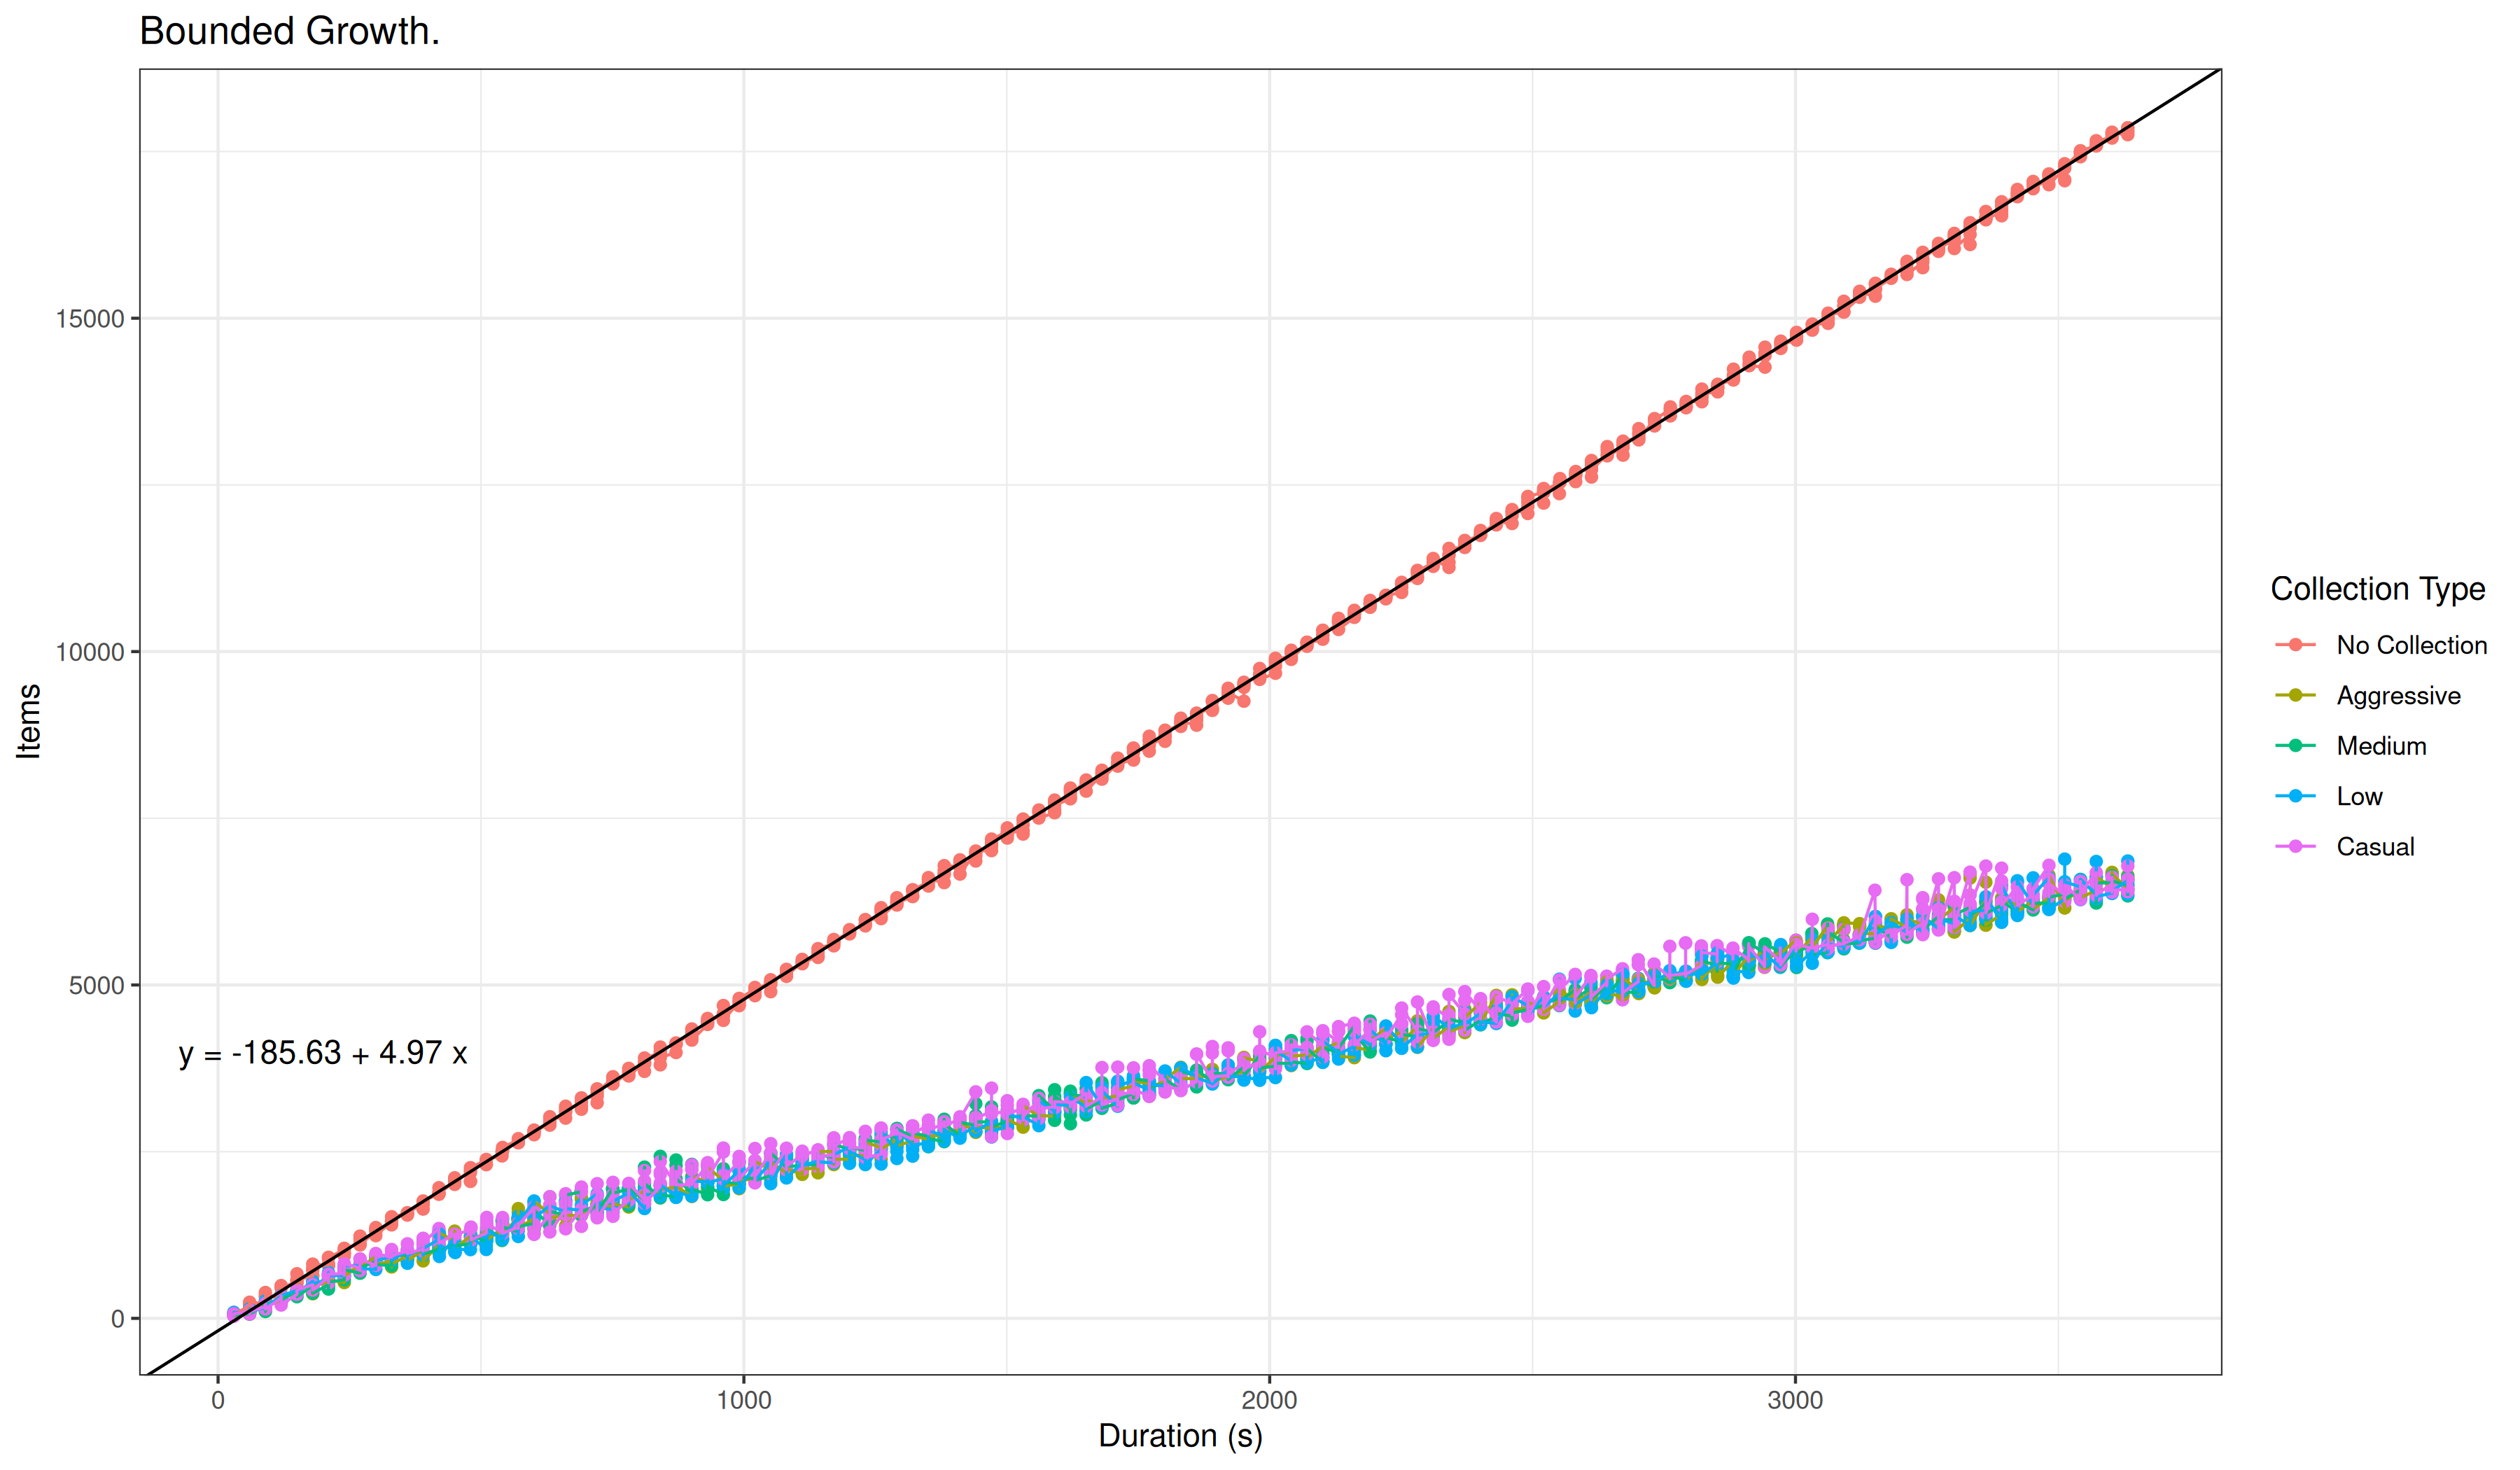
\includegraphics[width=\textwidth]{BoundedGrowth1_2}
\centering
\caption{With and without Garbage Collection.}
\label{fig:figureA}
\end{figure*}

\subsection*{Example Application: Distributed Text Editing}

One of the most classic examples of CRDTs in use is with a distributed
text editor. In order to achieve this a position value can be given to
each item of the set \cite{kleppmann_conflict-free_2017}. If we give an
absolute position to a character then a merge with another node may
leave newly added items in a location that does not make sense anymore.
The solution is to use an OR-Set and add the id of the previous item to
each item. This creates a sort of linked list including items who have
been replaced with a tombstone. When two items point to the same parent
we know there has been a conflict and implementations will usually
display one entire string first then the other. One node may add a word
after another that has been deleted synchronously. In this case, once
the two merge the first word will be replaced with a tombstone and not
displayed to the user but will still be present and can be referenced
by the new word; holding its position correctly. As a side-effect the
garbage collection algorithms need additional logic in order to work
with this solution.

\section*{Primary Objective}

To measure the memory reduction of using garbage collection in
combination with an OR-Set while keeping the properties of a
Conflict-free Replicated Data Type. Limited to 1.5 person weeks over
12 weeks.

\begin{figure*}[t]
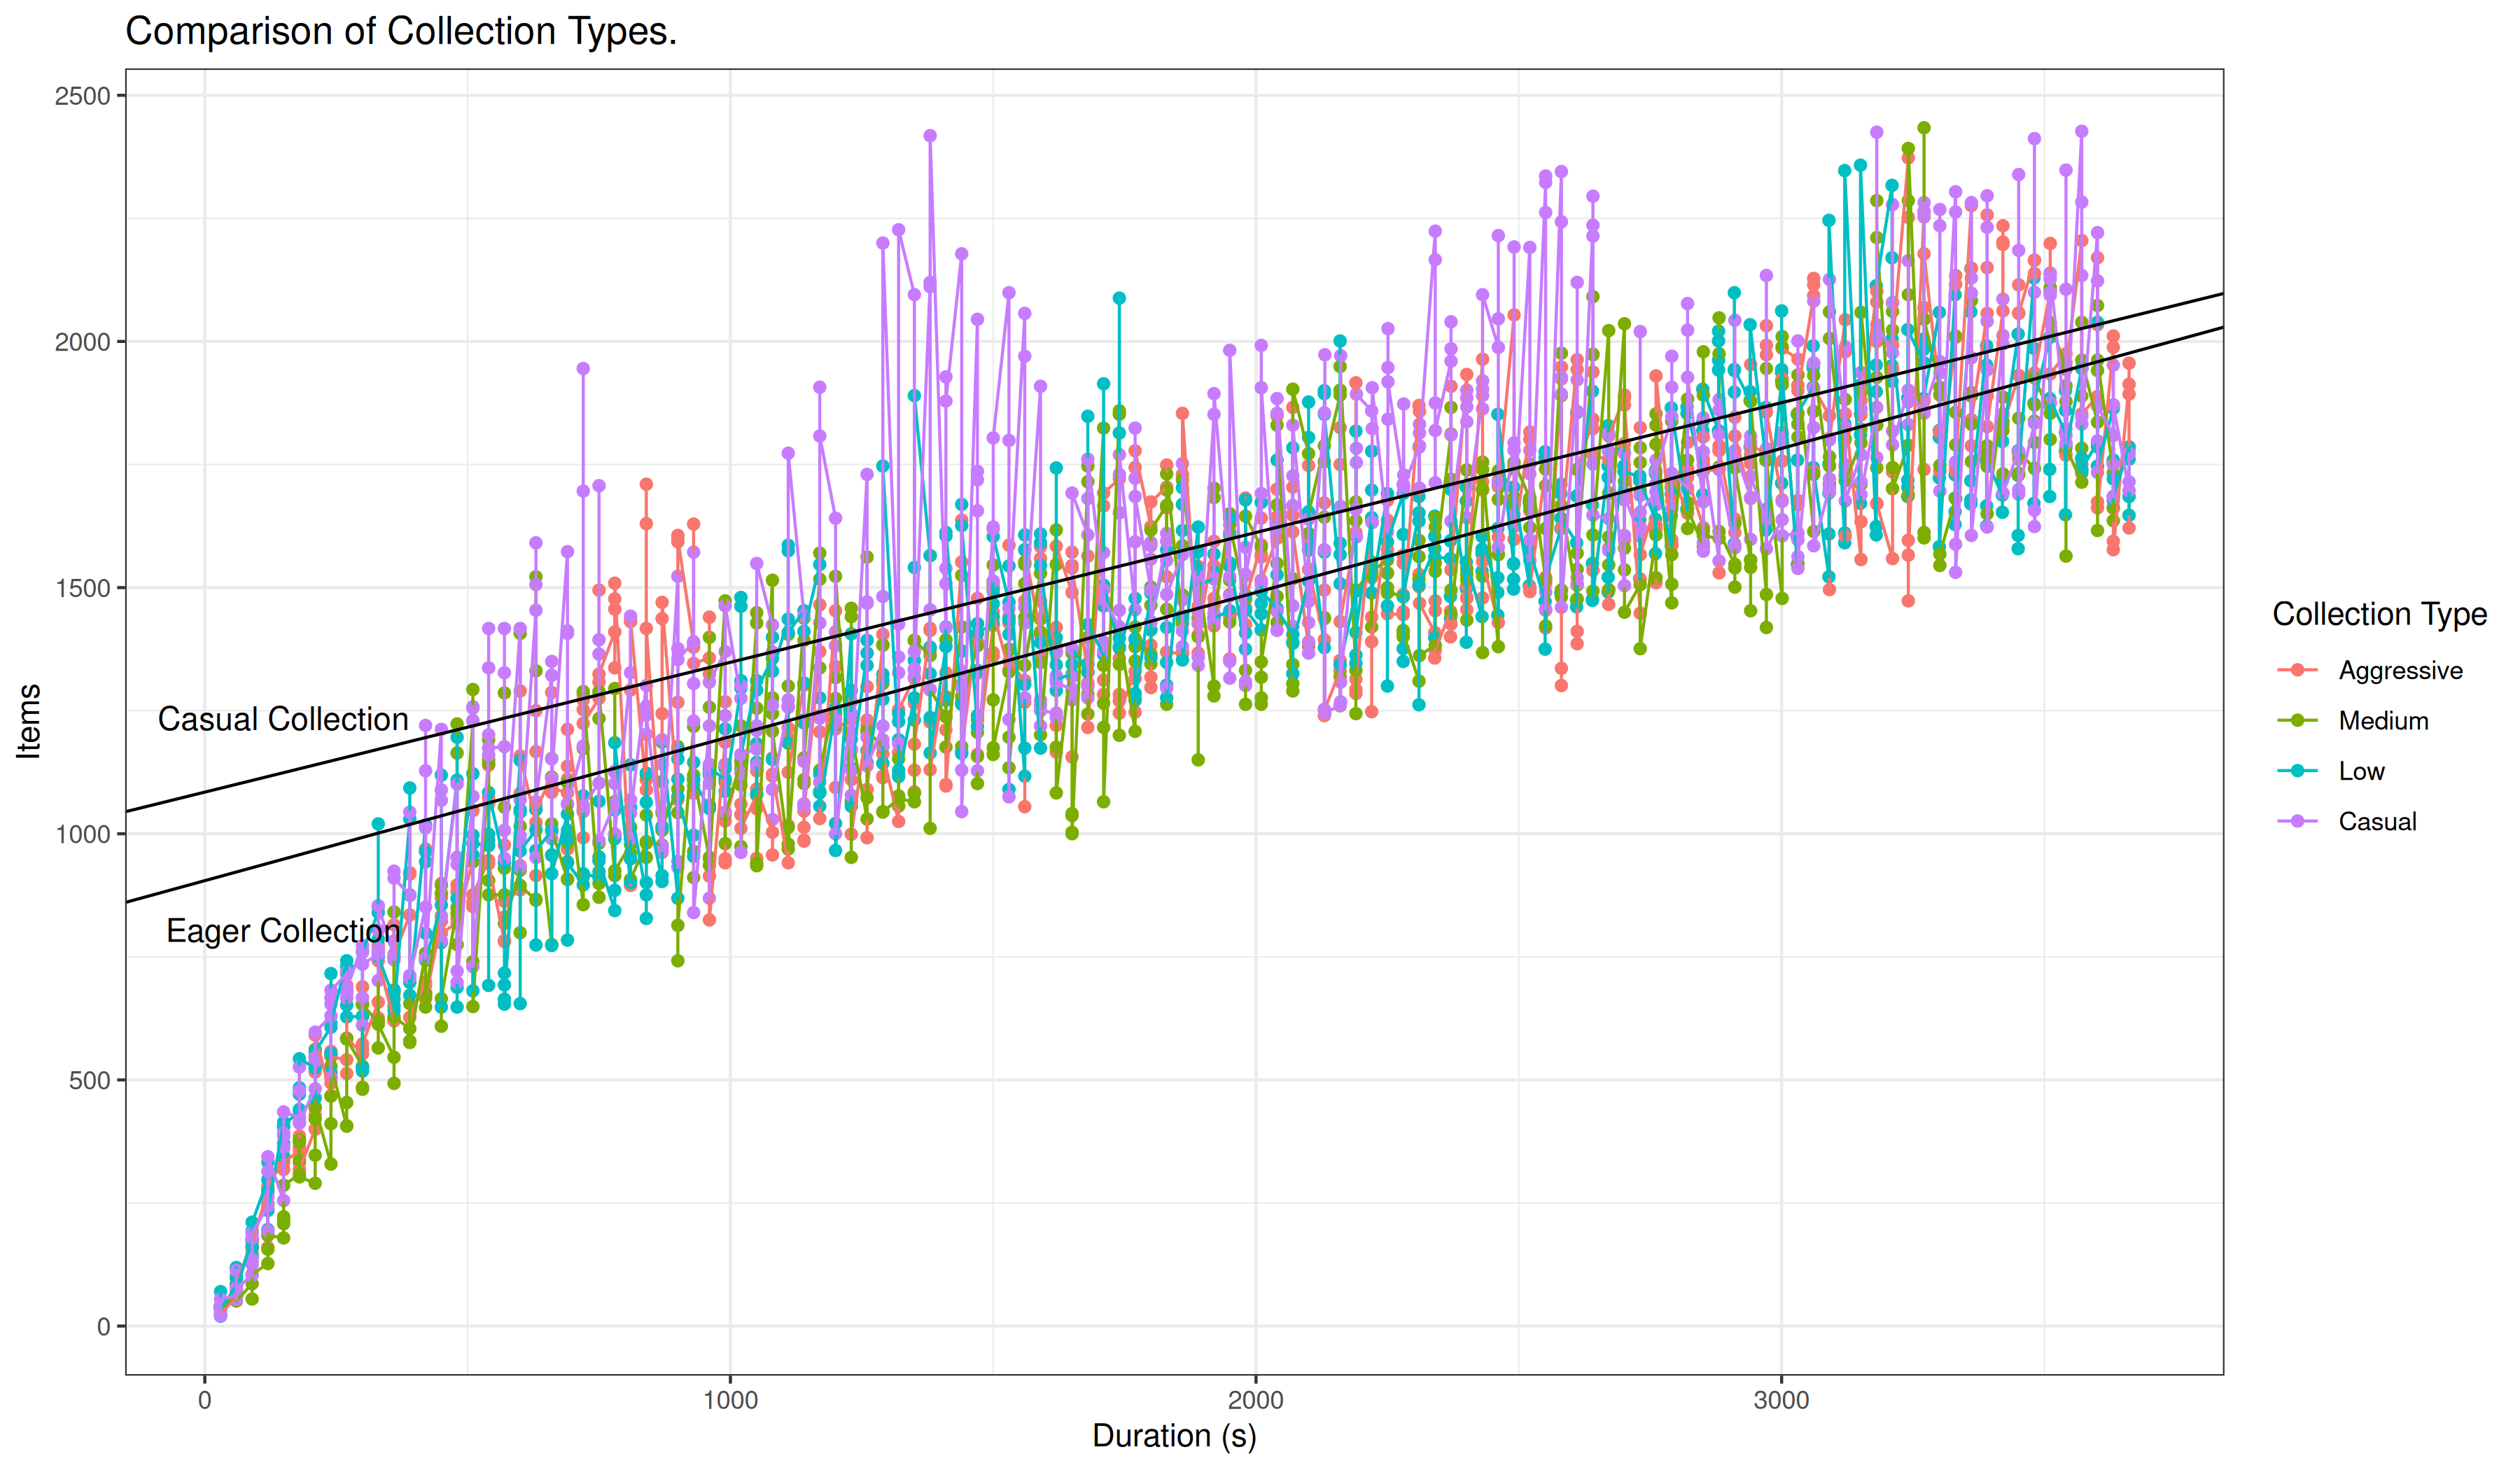
\includegraphics[width=\textwidth]{CollectionType3_1}
\centering
\caption{Comparison of Collection Types.}
\label{fig:figureB}
\end{figure*}

\section*{Solution Description}

In order to meet the requirements of the solution description software
was written to implement an OR-Set, its merging algorithm, and both
garbage collection algorithms. The implementation is written in C and
expects to be one node in a network of peers running the same software.
The OR-Set data type exposes an interface as described below:

Notation:
$ operation\_name(input) => Output $

$ add(data) => unique\_key $ \\
$ remove(unique\_key) => tombstone\_key $ \\
$ merge(local\_set, other\_set) $

Keys (both unique, item keys and tombstone keys) are 64 bit unsigned
integers. The first 8 bits are reserved for the origination node id. So
each node begins it's count at 1 + bitshift\_left(node\_id, 56). A unique item id is
generated from this number by adding 2 to this number after use. To
distinguish a tombstone id from an item id; even and odd numbers are
used respectively. The value assigned to that tombstone id is the item
id it removes.

The merge operation loops over every item in other\_set (making it a
O(N) operation). If the item is a regular item and is not in local\_set
then add it to local\_set. If the item is a tombstone then add the
tombstone to local\_set (if not already) and delete the id it was
assigned to delete.

As an important note, this implementation does not remove the id
completely from the set on a remove operation but rather replaces it to
a magic value (i.e. NULL) to prevent the merge operation from becoming
a O(n*m) operation.

The casual garbage collection algorithms works as a wrapper around the merge
operation. Casual collection first removes items it has already seen in
other\_set. Then it removes tombstones that are no longer needed in
local\_set. Eager collection works independently to track and push
casualty information.

\section*{Hypothesis}

\begin{itemize}
    \item While the data size of a nodes not using garbage collection will
          grow linearly with the amount of operations; using garbage collection
          will eventually be bounded if the dataset is bounded.
    \item An increase in garbage collection rate will lead to a decrease in
          total items at a given time.
\end{itemize}

\subsection*{Goals Tree}

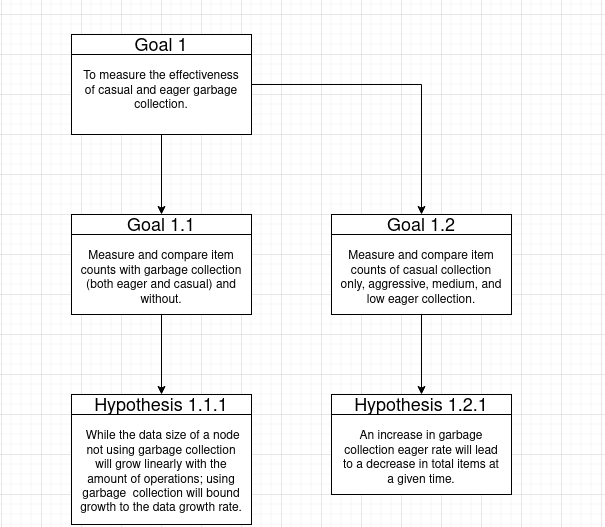
\includegraphics[width=\columnwidth]{GoalTree}

\section*{Experiment Design}

In order to draw a conclusion on our hypothesis one must be able to
track the number of items in a node at a given time. This was our only
response variable while we had many explanatory variables. These include
merge rate (how often a node will merge with another), number of nodes,
eager rate (how often an eager collection request will occur), and time.
We wanted to keep network reliability consistent so all tests were done
on a single machine.

\section*{Results}

Our first hypothesis questions the growth rate of our system with garbage
collection and without. It asserts that without garbage collection
growth rate will be equal to the operation rate. All of our tests use
an operation rate of 5 (1 per node with 5 nodes) so the growth rate
should be 5. With garbage collection the growth rate should be equal to
the growth rate of the data. All of our test use the same pattern for
each operation. First and second operation each node adds an item while
the third each node removes an item. This makes the growth rate of our
$1/3 * 5$ or $5/3$. Both of these match figure 1.


The next hypothesis questions the effectiveness of increasing collection
levels. In figure 2 we compare casual collection to eager collection. As
you can see at every point in our domain casual collection carries more
extra garbage then the more aggressive eager collection algorithms.
In this test casual collection holds about 4.4\% more garbage then eager
collection at X = 1000. Interestingly over time this difference shrinks.

\section*{Conclusion}

This paper has served to introduce topics from the concept of
Conflict-free Replicated Data Types with a focus on memory efficiency.
As well as present our research into the effectiveness of two garbage
collection algorithms. We can conclude from that research that:

\begin{enumerate}
    \item The growth rate of an OrSet using either garbage
        collection algorithm is based on the growth rate of
        the data as opposed to the operation rate.
    \bigskip
    \item The difference between casual collection and eager
        collection can be seen through a shrinking difference in
        items over time.
\end{enumerate}

\section*{Future Research}

With limited time and resources we were not able to answer every
question related to the area of garbage collection in CRDTs. Below is a
list of possible future research:

\begin{enumerate}
    \item Test which eager collection rate are best when
        balanced with network overhead.
    \bigskip
    \item Explore why the gap between casual collection and eager
        collection closes over time.
    \bigskip
    \item Prove and verify an OrSet network joining model that
        is compatibile with both eager and casual collection.
    \bigskip
    \item Measure garbage collection performance in a clustered
        network topology.
\end{enumerate}
% Future Research

\printbibliography[title=References]

\end{refsection}

\end{multicols}

\end{document}
